\documentclass{article}

% Conditional compilation.
% NOTE: If you set fullversionfalse, just compile ONCE so that TOC stays unchanged.
\newif\iffullversion
\fullversiontrue
%\fullversionfalse


%%%%%%%%%%%%%%%%%%%%%%%%%%%%%%%%%%%%%%%%%%%%%%%%%%%%%%%%%%%%%%%%%%%%%%%%%
\pagestyle{plain}                                                      %%
%%%%%%%%%% EXACT 1in MARGINS %%%%%%%                                   %%
\setlength{\textwidth}{6.5in}     %%                                   %%
\setlength{\oddsidemargin}{0in}   %% (It is recommended that you       %%
\setlength{\evensidemargin}{0in}  %%  not change these parameters,     %%
\setlength{\textheight}{8.5in}    %%  at the risk of having your       %%
\setlength{\topmargin}{0in}       %%  proposal dismissed on the basis  %%
\setlength{\headheight}{0in}      %%  of incorrect formatting!!!)      %%
\setlength{\headsep}{0in}         %%                                   %%
\setlength{\footskip}{.5in}       %%                                   %%
%%%%%%%%%%%%%%%%%%%%%%%%%%%%%%%%%%%%                                   %%
\newcommand{\required}[1]{\section*{\hfil #1\hfil}}                    %%
\renewcommand{\refname}{\hfil References Cited\hfil}                   %%
\bibliographystyle{plain}                                              %%
%%%%%%%%%%%%%%%%%%%%%%%%%%%%%%%%%%%%%%%%%%%%%%%%%%%%%%%%%%%%%%%%%%%%%%%%%

\usepackage{graphicx}
\usepackage{color}

\pagestyle{empty}


\usepackage{fancyvrb}

\newenvironment{bluecode}{\VerbatimEnvironment \color{blue} \begin{Verbatim}}
{\end{Verbatim}}


\begin{document}

\large

\vbox{}
\begin{figure}[!ht]
%\hspace{-4mm}

\includegraphics[width=8cm]{img/logo.png}
\vspace{18mm}
\end{figure}

\begin{figure}[!ht]
\begin{center}
%\hspace{-4mm}
%\hspace{-20mm}
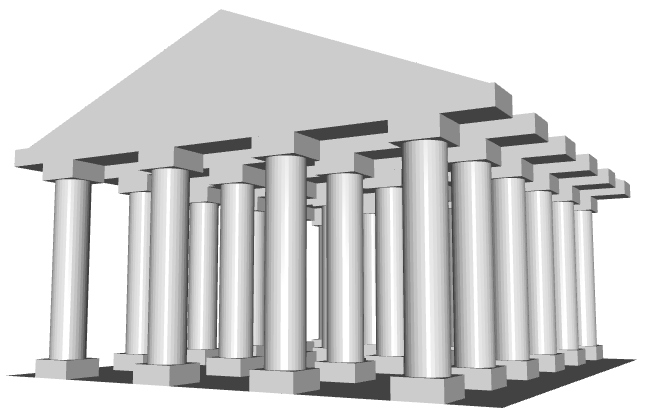
\includegraphics[width=8cm]{img/plasm-temple.png}\hspace{1cm}
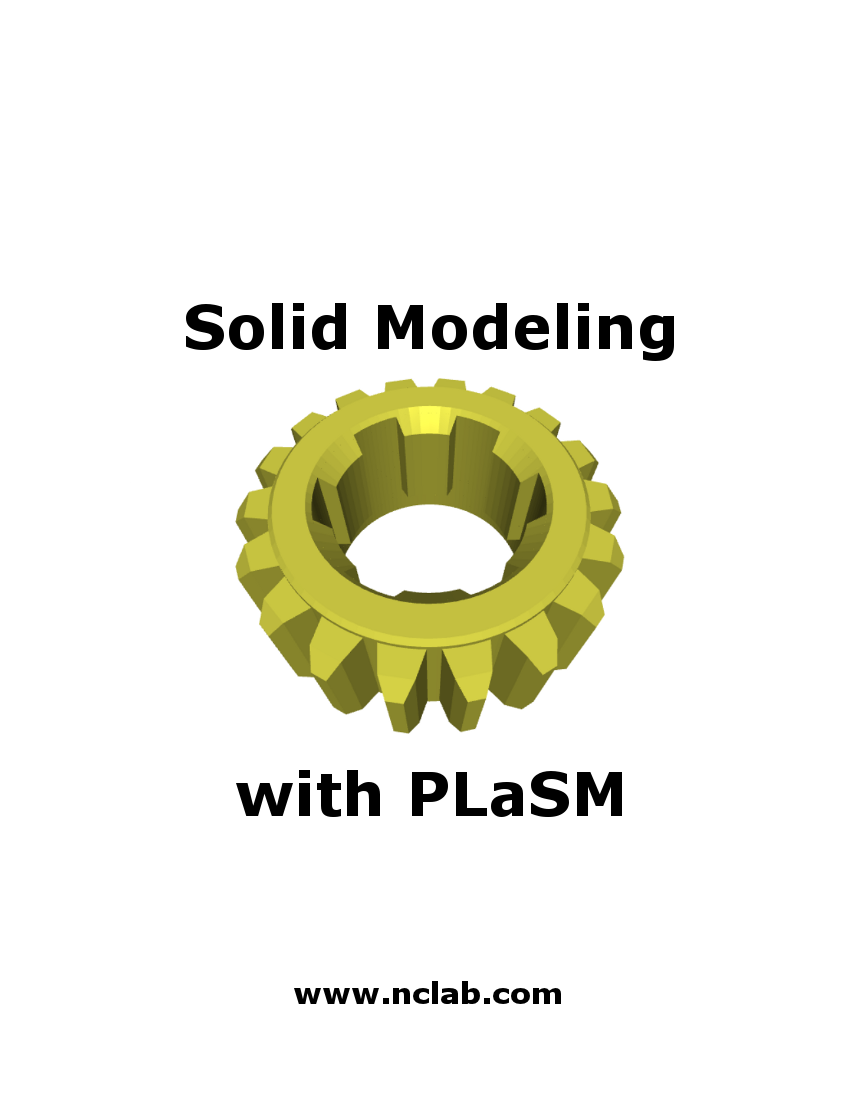
\includegraphics[width=5.5cm]{img/plasm-frontpage.png}
\vspace{15mm}
\end{center}
\end{figure}

\begin{center}
{\Huge \bf Review Questions}\\
\vbox{}
\vspace{1.4cm}
\iffullversion
\else
\centerline{\huge \color{red}{PREVIEW}}
\fi
\vfill
{\large
{\bf Pavel Solin \& Alberto Paoluzzi}
}
\end{center}
\vfill
\vfill
\begin{center}
Copyright 2012 FEMhub Inc. All rights reserved.
\end{center}
\newpage
\hbox{}
%%%%%%%%%%%%%%%%%%%%%%%%%%%%%%%%%%%%%%%%%%%%%%%%%%%%%%%%%%%%%%%%%%%%%%%%%


\newpage
%{\ }
\setcounter{tocdepth}{2}
\tableofcontents
%\pagestyle{plain}


%%%%%%%%%%%%%%%%%%%%%%%%%%%%%%%%%%%%%%%%%%%%%%%%%%%%%%%%%%%%%%%%%%%%%%%%%
\newpage

\pagestyle{plain}
\setcounter{page}{1}

\section{Getting Started}

\subsection{Review questions}

\begin{enumerate}
\item How does Solid Modeling differ from Computer Graphics?
\begin{itemize}
\item[A1] There is no difference, they are the same thing. 
\item[A2] Computer graphics represents 3D onjects more precisely.
\item[A3] Solid Modeling represents 3D objects more precisely.
\item[A4] Solid Modeling is used primarily for 3D animations.
\end{itemize}
\item What does the abbreviation CAD stand for?
\begin{itemize}
\item[A1] Computer-assisted drawing.
\item[A2] Computer-allowed discrepancy.
\item[A3] Computer-aided design.
\item[A4] Computer-amplified drumming.
\end{itemize}
\item What is PLaSM?
\begin{itemize}
\item[A1] Make of plasma 3D TVs.
\item[A2] Computer graphics library.
\item[A3] Design language backed up with powerful computational geometry algorithms.
\item[A4] Browser plugin for rendering 3D objects.
\end{itemize}
\item In NCLab, scripts are evaluated:
\begin{itemize}
\item[A1] On the user's computer.
\item[A2] In the user's web browser.
\item[A3] On a remote server.
\item[A4] Using the user's graphic card.
\end{itemize}
\item How can a PLaSM script be evaluated?
\begin{itemize}
\item[A1] By hitting ENTER.
\item[A2] By clicking on the green arrow under the input cell.
\item[A3] By clicking on the green arrow in the upper menu.
\item[A4] By clicking on Run in the File menu.
\end{itemize}
\item What of the following is the correct way to create a cube of edge length $e$?
\begin{itemize}
\item[A1] {\tt c = C(e)}
\item[A2] {\tt c = CB(e)}
\item[A3] {\tt c = CUBE(e)}
\item[A4] {\tt c = HEXAHEDRON(e)}
\end{itemize}
\item What color is represented by the triplet [0, 0, 0]?
\begin{itemize}
\item[A1] Black
\item[A2] White
\item[A3] Green
\item[A4] Magenta.
\end{itemize}
\end{enumerate}

\section{Creating Simple Objects}

\subsection{Review questions}

\begin{enumerate}
\item Coming soon.
\begin{itemize}
\item[A1]
\item[A2]
\item[A3]
\item[A4]
\end{itemize}
\end{enumerate}

\section{Basic Transformations}

\subsection{Review questions}

\begin{enumerate}
\item Coming soon.
\begin{itemize}
\item[A1]
\item[A2]
\item[A3]
\item[A4]
\end{itemize}
\end{enumerate}


\section{Boolean Operations}


\subsection{Review questions}

\begin{enumerate}
\item Coming soon.
\begin{itemize}
\item[A1]
\item[A2]
\item[A3]
\item[A4]
\end{itemize}
\end{enumerate}


\section{Creating Simple Objects (Continued)} \label{sec:cso2}


\subsection{Review questions}

\begin{enumerate}
\item Coming soon.
\begin{itemize}
\item[A1]
\item[A2]
\item[A3]
\item[A4]
\end{itemize}
\end{enumerate}


\section{Curves and Curved Surfaces}\label{sec:curves}


\subsection{Review questions}

\begin{enumerate}
\item Coming soon.
\begin{itemize}
\item[A1]
\item[A2]
\item[A3]
\item[A4]
\end{itemize}
\end{enumerate}


\section{The Power of Scripting}


\subsection{Review questions}

\begin{enumerate}
\item Coming soon.
\begin{itemize}
\item[A1]
\item[A2]
\item[A3]
\item[A4]
\end{itemize}
\end{enumerate}

\section{Advanced Techniques}

\subsection{Review questions}

\begin{enumerate}
\item Coming soon.
\begin{itemize}
\item[A1]
\item[A2]
\item[A3]
\item[A4]
\end{itemize}
\end{enumerate}

\end{document}
